\documentclass[pdflatex,sn-basic,Numbered]{sn-jnl}

\usepackage{graphicx}
\usepackage{booktabs}
\usepackage{amsmath,amssymb}
\usepackage{microtype}
\usepackage{xcolor}
\usepackage{hyperref}
\usepackage{tikz}
\usepackage{algorithm}
\usepackage{algpseudocode}
\usetikzlibrary{arrows.meta,positioning,fit,backgrounds}
\hypersetup{colorlinks=true,linkcolor=blue,citecolor=blue,urlcolor=blue}
\graphicspath{{final/figures/}}

\newcommand{\AIA}{\operatorname{AIA}}
\newcommand{\NDCG}{\operatorname{NDCG}}
\newcommand{\Recall}{\operatorname{Recall}}
\newcommand{\MRR}{\operatorname{MRR}}
\newcommand{\safeinput}[1]{\IfFileExists{#1}{\input{#1}}{}}

\title[ActionShap]{ActionShap: Beyond Deletion Faithfulness toward Intervention-Robust Recommendation Explanations}

\author*[1]{\fnm{Mouad} \sur{Louhichi}}\email{mouad.louhichi@um5.ac.ma}
\author[1]{\fnm{Redwane} \sur{Nesmaoui}}
\author[1]{\fnm{Mohamed} \sur{Lazaar}}
\affil[1]{\orgdiv{National Higher School of Computer Science and Systems Analysis (ENSIAS)}, \orgname{Mohammed V University in Rabat}, \orgaddress{\city{Rabat}, \country{Morocco}}}

\begin{document}
\maketitle

\begin{abstract}
Recommendation explanations are commonly evaluated by deleting historical interactions, although deployed recommendation systems act through bounded changes to the influence of observed evidence. Deletion and feasible intervention therefore measure different properties. We introduce \textbf{ActionShap}, a model-agnostic protocol for evaluating whether user-specific explanation rankings predict the effects of declared, system-executable interventions. ActionShap separates deletion alignment, bounded-intervention alignment, and the quality of the joint action selected under a fixed budget. It fixes temporal splits, complete pre-test-history exclusion, target-plus-unseen-negative candidate sets, global tie priorities, signed action selection, abstention, convergence, and inference over distinct users. We evaluate Monte Carlo Shapley, locally weighted LIME, leave-one-out, greedy sequential deletion, and a random control on MovieLens-1M and Amazon Digital Music. The primary analysis uses a history-conditioned ItemKNN recommender, 1,000 users, five common seeds, and exact budget-two oracles; a latent profile model and full-unseen-catalogue subset provide robustness evidence. Shapley improves from deletion to bounded target-margin alignment in the primary ItemKNN conditions, with gaps of $+0.0169$ on MovieLens and $+0.1285$ on Amazon, but local methods retain higher absolute alignment and slightly better MovieLens NDCG decisions. The random control remains near its within-user null, showing that a positive gap alone is not evidence of explanation validity. ActionShap contributes an auditable evaluation instrument for separating perturbation sensitivity, absolute alignment, and intervention decision quality rather than claiming universal superiority for any explainer.
\end{abstract}

\keywords{explainable recommendation \and intervention evaluation \and faithfulness \and actionability \and Shapley value \and LIME \and counterfactual recommendation}

\section{Introduction}
An explanation is often consumed as advice about where to act. A user, analyst, or system operator does not usually ask only whether a recommendation score changes when an input is deleted; they ask what will happen if a factor is discounted, suppressed, or otherwise modified within an available operating policy. The distinction is important in recommender systems because historical interactions are evidence, not necessarily controls. Removing an interaction can be a useful faithfulness diagnostic while being an unrealistic intervention.

This paper studies the resulting evaluation gap. We ask whether an attribution ranking predicts the effect of a feasible modification to the interaction history, and whether the explanation leads to a useful joint intervention under a fixed budget. The question is deliberately narrower than recourse: ActionShap does not claim that a user can cause a profile change, does not estimate causal effects in the world, and does not propose a new recommender architecture. It audits an explanation inside a frozen recommender and an explicitly declared intervention simulator.

The protocol is motivated by three observations. First, deletion and bounded modification are different estimands. A deletion moves a factor to a baseline that may be far outside an operational range. Second, pointwise attribution quality does not determine decision quality: a method can rank individual effects well while selecting a harmful pair, or select a good pair despite modest average rank agreement. Third, a method comparison is not interpretable without a chance control, valid-user counts, convergence diagnostics, and inference over distinct users rather than repeated seed--user records.

ActionShap addresses these issues with a history-conditioned interaction-player game. For each user, the most recent training interactions form the player set. A frozen ItemKNN model computes scores from the retained history at inference time, allowing masking and bounded downweighting to change the profile without retraining. The primary characteristic function is a continuous target-margin utility selected by an independent convergence study; NDCG@10 remains the operational ranking outcome. Every method receives the same temporal users, candidates, intervention strengths, action space, and tie rules.

Our contributions are fourfold:
\begin{enumerate}
  \item We formalize a recommendation-specific evaluation protocol that separates deletion faithfulness, bounded intervention, and budgeted decision quality under a frozen model.
  \item We provide complementary magnitude, signed-direction, success, abstention, regret, stability, and within-user null metrics, with explicit handling of constant vectors and inactive oracles.
  \item We give executable algorithms for paired Monte Carlo attribution, signed action selection, the exact $B\le2$ oracle, user-level inference, and independent convergence selection.
  \item We report a two-dataset, two-model, five-seed benchmark. The primary ItemKNN results show that Shapley can improve relative to deletion while LIME and LOO retain higher absolute alignment and downstream decision quality in some conditions.
\end{enumerate}

The paper makes no a priori claim that Shapley, LIME, LOO, or any other explainer is best. The framework is the contribution; method rankings are empirical and bounded by the declared offline simulator.

\begin{figure}[t]
\centering
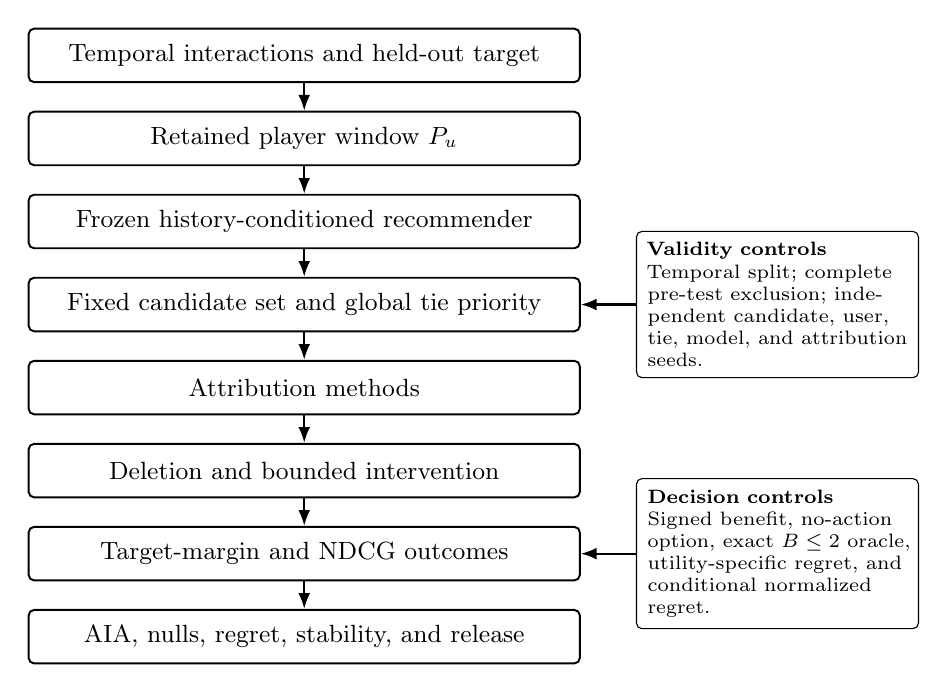
\begin{tikzpicture}[
  stage/.style={draw=black, fill=white, rounded corners=2pt, minimum width=7cm, minimum height=0.68cm, align=center, font=\small, line width=.7pt},
  edge/.style={-{Latex[length=2mm]}, draw=black, line width=.8pt},
  note/.style={draw=black, fill=white, rounded corners=2pt, align=left, font=\scriptsize, inner sep=4pt}
]
\node[stage] (a) {Temporal interactions and held-out target};
\node[stage, below=3.5mm of a] (b) {Retained player window $P_u$};
\node[stage, below=3.5mm of b] (c) {Frozen history-conditioned recommender};
\node[stage, below=3.5mm of c] (d) {Fixed candidate set and global tie priority};
\node[stage, below=3.5mm of d] (e) {Attribution methods};
\node[stage, below=3.5mm of e] (f) {Deletion and bounded intervention};
\node[stage, below=3.5mm of f] (g) {Target-margin and NDCG outcomes};
\node[stage, below=3.5mm of g] (h) {AIA, nulls, regret, stability, and release};
\foreach \x/\y in {a/b,b/c,c/d,d/e,e/f,f/g,g/h}{\draw[edge] (\x)--(\y);}
\node[note, right=7mm of d, text width=3.3cm] (v) {\textbf{Validity controls}\\Temporal split; complete pre-test exclusion; independent candidate, user, tie, model, and attribution seeds.};
\draw[edge] (v.west)--++(-4mm,0)|-(d.east);
\node[note, right=7mm of g, text width=3.3cm] (q) {\textbf{Decision controls}\\Signed benefit, no-action option, exact $B\le2$ oracle, utility-specific regret, and conditional normalized regret.};
\draw[edge] (q.west)--++(-4mm,0)|-(g.east);
\end{tikzpicture}
\caption{ActionShap evaluation architecture. The fixed vertical path separates player construction, model scoring, attribution, intervention execution, and outcome measurement. Side panels show controls held constant across methods.}
\label{fig:architecture}
\end{figure}

\section{Related Work}
\subsection{Explainable recommendation}
Explainable recommendation includes feature, item, path, attention, sentiment, and natural-language rationales. Surveys emphasize that these forms serve different objectives, including user persuasion, model fidelity, transparency, and preference communication \citep{zhang2020survey}. Latent-factor explanations expose item or feature contributions, while post-hoc methods apply model-agnostic surrogates such as LIME and SHAP \citep{peake2018,nobrega2019,ribeiro2016,lundberg2017}. Sentiment- and phrase-level models construct explanations during recommendation rather than evaluating a post-hoc attribution \citep{zhang2014,zheng2018}. ActionShap addresses a complementary question: whether an explanation predicts the outcome of a declared feasible change.

\subsection{Recommender models and offline evaluation}
Classical matrix factorization and pairwise learning-to-rank remain foundations for offline recommendation \citep{koren2009,joachims2002,rendle2009,burges2005}. Neural collaborative filtering, recurrent session models, self-attentive sequence models, and bidirectional transformer recommenders broaden the architecture space \citep{he2017ncf,hidasi2016gru4rec,kang2018sasrec,sun2019bert4rec}. Graph recommenders introduce a further distinction between a trained graph representation and an inference-time profile intervention \citep{wang2019ngcf,he2020lightgcn}. We use ItemKNN as the primary model because its history dependence is transparent under masking; the profile aggregator is a robustness model, not a claim to cover all architectures.

Offline evaluation depends on temporal leakage, negative sampling, exposure, and the candidate universe. Results on a target-plus-negative set are sampled-ranking results, not catalogue retrieval. Evaluation choices can materially change rankings between methods and models \citep{harper2016,bennett2007,zheng2017,saito2021,ji2020,chen2022,mcnamara2017}. ActionShap fixes these choices before final testing, reports popularity references, and separates sampled ranking from full-unseen-catalogue evaluation.

\subsection{Faithfulness, counterfactual evaluation, and recourse}
Deletion and insertion tests measure model dependence but can be sensitive to the baseline and perturbation path. Sanity checks show that some attribution maps can appear plausible while failing model or data randomization tests \citep{adebayo2018}. Perturbation-based explanations also raise the question of whether the perturbation remains within a meaningful data manifold \citep{hooker2019}. Counterfactual recommendation and recourse methods instead search for profile or graph changes that alter a ranking or decision \citep{ghazimatin2020,tran2021,tan2021,yao2022,baklanov2024,barkan2024,gurevitch2025,mohammadi2025,nguyen2026,wachter2017,karimi2021}. ActionShap does not generate causal recourse. It evaluates an attribution under a fixed intervention policy and makes the policy, cost, authority, and offline limitations explicit.

\subsection{Interpretable machine learning and cooperative attribution}
Interpretability is not a single property: faithfulness, stability, simulatability, and usefulness can disagree \citep{gilpin2018,arrieta2020,molnar2022,samek2017,deyoung2020}. SHAP connects feature attribution with cooperative-game values, while sampling makes the construction applicable when exact enumeration is infeasible \citep{shapley1953,castro2009,lundberg2020,covert2021}. ActionShap treats Shapley as one interchangeable explainer. Its axioms do not imply causal validity, intervention feasibility, or decision superiority; these are measured separately.

\begin{table}[t]
\centering
\small
\caption{Positioning by evaluation target.}
\label{tab:positioning}
\begin{tabular}{lcccc}
\toprule
Approach & Explainer audit & Feasible policy & Joint regret & Abstention\\
\midrule
Deletion/insertion & Yes & No & No & No\\
Counterfactual explanation & Usually generates & Method-specific & Sometimes & Method-specific\\
Algorithmic recourse & No & Yes & Optimization target & Often\\
ActionShap & Yes & Yes & Yes & Yes\\
\bottomrule
\end{tabular}
\end{table}

\section{Problem Formulation}
\subsection{Temporal user-specific game}
For user $u$, let $H_u^{\mathrm{train}}$ contain interactions before validation and test. The player set is the most recent training window,
\begin{equation}
P_u=\{p_{u1},\ldots,p_{un_u}\},\qquad n_u\le n_{\max}=20.
\end{equation}
Interactions are ordered by $(\mathrm{timestamp},\mathrm{original\_record\_index})$; the last event is test and the preceding event is validation. Validation and test events are never players. Models are fitted using complete training histories; the cap limits only the explanation game.

Every user has a fixed candidate set $E_u$ containing the held-out target and sampled negatives. Negatives exclude the complete pre-test history, including validation. The user seed, candidate seed, tie seed, model seed, and attribution seed are independent. Full-catalogue robustness uses the target plus all unseen items. Target coverage is one by construction and is not called retrieval recall.

\subsection{History-conditioned recommenders}
The primary ItemKNN score is a weighted mean of frozen item--item similarities:
\begin{equation}
f_u^S(i)=
\begin{cases}
\displaystyle\frac{\sum_{h\in S}w_hs(i,h)}{\sum_{h\in S}w_h},&S\ne\varnothing,\\[6pt]
0,&S=\varnothing.
\end{cases}
\end{equation}
A profile aggregator is used for robustness,
\begin{equation}
p_u(S)=
\begin{cases}
\displaystyle\frac{\sum_{h\in S}w_hq_h}{\sum_{h\in S}w_h},&S\ne\varnothing,\\[6pt]
\mathbf 0,&S=\varnothing,
\end{cases}
\qquad f_u^S(i)=q_i^\top p_u(S).
\end{equation}
Its item embeddings are trained once with a leave-one-out BPR-style objective and then frozen. Static user embeddings are excluded from attribution because post-training history masking cannot change their scores.

\subsection{Utilities and interventions}
The primary characteristic function is the target-margin utility
\begin{equation}
v_u^{\mathrm{attr}}(S)=\sigma\left(s_y^S-\frac{1}{L}\sum_{i\in\operatorname{TopL}_{-y}}s_i^S\right),
\end{equation}
where $y$ is the temporal target. The operational ranking outcome is
\begin{equation}
q_u(S)=\NDCG@10(f_u^S,y).
\end{equation}
All effects and regrets are stored separately for target margin and NDCG. The empty coalition has target-margin utility $0.5$ and deterministic catalogue ties.

Deletion is the diagnostic $w_p\leftarrow0$. The primary feasible intervention is bounded downweighting,
\begin{equation}
\operatorname{do}(p;\rho):w_p\leftarrow\rho w_p,\qquad \rho=0.5,
\end{equation}
with $\rho=0.25$ as a predeclared sensitivity. No model retraining occurs after an intervention.

The action space is
\begin{equation}
\mathcal A_{u,B}=\{A\subseteq P_u:|A|\le B\},
\end{equation}
including no action. The primary scientific budget is $B=2$. A signed attribution predicts downweighting benefit as $-\phi$; only positive predicted benefit is selected. LOO is an algebraic deletion oracle at $B=1$, not a headline competitor.

\section{ActionShap Protocol}
\subsection{Attribution methods}
For permutation $\pi$, let $S_{p,\pi}$ be the predecessor coalition of player $p$. The Monte Carlo Shapley estimate is
\begin{equation}
\widehat\phi_{u,p}=\frac{1}{M}\sum_{m=1}^{M}\left[v(S_{p,\pi_m}\cup\{p\})-v(S_{p,\pi_m})\right].
\end{equation}
Reverse orders are paired and coalition states are cached. The comparison includes locally weighted binary-mask LIME, LOO, greedy sequential deletion, and random attribution. No method observes measured intervention effects, oracle actions, or aggregate test outcomes.

\subsection{Metrics}
Magnitude AIA is
\begin{equation}
\AIA_u(g)=\operatorname{Spearman}(|\phi^g_{u,p}|,|\Delta^{\mathrm{attr}}_{u,p}|).
\end{equation}
Deletion AIA and bounded AIA are reported separately; their difference is the Actionability Gap. Signed alignment compares $-\phi$ with signed intervention effects. We also report direction accuracy, top-$k$ precision, realized effect, success, harm, abstention, and stability.

For each user and seed, 1,000 within-user permutations shuffle effect magnitudes across players. We report null means, null 95th percentiles, plus-one permutation $p$-values, and valid-user counts. Constant vectors are missing, not imputed.

\subsection{Decision quality and regret}
For utility $z$, the exact budget-two oracle is
\begin{equation}
A_u^{*,z}=\arg\max_{A\in\mathcal A_{u,2}}\Delta_u^z(A),
\end{equation}
and the method action is $\widehat A_{u,g}$. Regret is
\begin{equation}
\operatorname{Regret}_u^z(g)=\Delta_u^z(A_u^{*,z})-\Delta_u^z(\widehat A_{u,g}).
\end{equation}
Normalized regret is reported only when $\Delta_u^z(A_u^{*,z})>10^{-12}$ and is averaged conditionally over active-oracle users. It is not clipped; harmful actions may exceed one.

\begin{algorithm}[t]
\caption{Paired Monte Carlo attribution}
\label{alg:shapley}
\begin{algorithmic}[1]
\Require $u,P_u,v,M$, attribution seed
\Ensure $\widehat{\boldsymbol\phi}_u$
\State Initialise $\hat\phi_{u,p}\gets0$ for all $p\in P_u$
\For{$m=1$ to $M$}
\State Draw $\pi_m$ and its reverse; evaluate the cached prefix walk
\For{each consecutive pair $(S,S\cup\{p\})$}
\State $\hat\phi_{u,p}\gets\hat\phi_{u,p}+v(S\cup\{p\})-v(S)$
\EndFor
\EndFor
\State Average over orders and record finite/constant-vector flags
\end{algorithmic}
\end{algorithm}

\begin{algorithm}[t]
\caption{Signed action selection and exact budget-two oracle}
\label{alg:actions}
\begin{algorithmic}[1]
\Require $\hat{\boldsymbol\phi}_u$, profile weights, $\rho=0.5$, candidate set
\Ensure Method action and utility-specific oracle actions
\State Enumerate $\varnothing$, every singleton, and every pair
\For{each action $A$}
\State Apply $w_p\gets\rho w_p$ simultaneously for $p\in A$
\State Cache target-margin and NDCG effects
\EndFor
\State Select $\arg\max_A[-\sum_{p\in A}\hat\phi_{u,p}]$ over positive scores
\State Return $\varnothing$ when the best score is at most $10^{-12}$
\State Select the exact oracle separately for each utility
\end{algorithmic}
\end{algorithm}

\begin{algorithm}[t]
\caption{Distinct-user inference and AIA null}
\label{alg:inference}
\begin{algorithmic}[1]
\Require Five seed records per user and $R=1000$ null draws
\Ensure User-level estimates and corrected comparisons
\For{each distinct user $u$}
\State Average repeated seeds within $u$
\State Compute AIA only for finite, nonconstant vectors
\For{$r=1$ to $R$}
\State Shuffle effect magnitudes within $u$ and seed; recompute AIA
\EndFor
\EndFor
\State Bootstrap users; apply paired plus-one tests and Holm correction
\end{algorithmic}
\end{algorithm}

\begin{algorithm}[t]
\caption{Independent convergence selection}
\label{alg:convergence}
\begin{algorithmic}[1]
\Require $M\in\{25,50,100,250,500,1000\}$ and independent $M=1000$ reference
\Ensure Selected $M$ or explicit unconverged status
\For{each candidate $M$}
\State Compare attribution ranks and signed-$B=2$ action Jaccard with reference
\State Record rank-valid fraction and threshold coverage
\EndFor
\State Select smallest $M$ with rank $\ge.95$, Jaccard $\ge.80$, rank validity $\ge.95$
\If{no candidate qualifies}\State Retain $M=1000$ as unconverged stress test\EndIf
\end{algorithmic}
\end{algorithm}

\section{Experimental Protocol}
\subsection{Datasets and temporal split}
We use MovieLens-1M \citep{harper2016,ni2019} and Amazon Digital Music reconstructed from the Amazon Reviews 2018 release. Positive feedback is rating $\ge4$; Amazon duplicate user--item records retain the latest deterministic event and iterative 5-core filtering is reapplied after thresholding. MovieLens retains 6,035 users, 3,533 items, and 575,276 positive interactions. Amazon retains 10,623 users, 8,582 items, and 104,431 interactions. Source and processed hashes are recorded in the final manifest.

\subsection{Models, candidates, and gates}
The matrix includes ItemKNN and profile aggregation, five seeds, primary 1,000-user sampled ranking, 250-user full-catalogue subsets, and predeclared history, candidate, intervention-strength, budget, and utility sensitivities. ItemKNN passes all blocking masking gates. The profile model fails the NDCG masking threshold for one MovieLens seed (mean absolute change $0.000682$ versus $0.001$) and is retained as a nonblocking robustness boundary.

\subsection{Statistical analysis}
Seeds are averaged within distinct users before inference. We use user bootstrap intervals, paired plus-one sign permutations, effect sizes, and Holm correction within comparison families. We report missing correlations, active-oracle counts, and conditional normalized regret. No coalition evaluation is an independent statistical observation.

\subsection{Reproducibility}
The real result archive contains 80 recommendation runs plus five convergence studies. All assets in this manuscript are generated from schema-v2 raw results with repository-relative paths and content hashes. The primary ItemKNN target-margin analysis uses at least $M=500$ permutations; the independent convergence study selects lower diagnostic values for some conditions, while the conservative final floor is retained.

\section{Results}
All numerical claims below are generated only when `final/manifests/validation_report.json` reports PASS. The legacy pilot is excluded from the canonical package.

\subsection{Recommendation quality and protocol audit}
Table~\ref{tab:protocol-audit} shows that primary ItemKNN exceeds the popularity reference on both datasets. MovieLens ItemKNN reaches NDCG@10 $=0.284$ and Recall@10 $=0.504$, compared with $0.158$ and $0.320$ for popularity. Amazon ItemKNN reaches $0.181$ and $0.285$, compared with $0.090$ and $0.155$. The profile model is weaker on both datasets and is therefore interpreted only as architectural robustness evidence.

\safeinput{final/tables/protocol_audit.tex}

\subsection{Faithfulness versus bounded alignment}
Table~\ref{tab:aia-components} separates deletion AIA, bounded AIA, and their difference. On MovieLens ItemKNN, Shapley has bounded AIA $0.779$ versus $0.933$ for LIME and $0.978$ for LOO. On Amazon, Shapley has bounded AIA $0.414$ versus $0.827$ and $0.851$. Thus Shapley does not win absolute alignment.

The contrast is in the change between perturbations. Shapley’s primary gap is $+0.0169$ on MovieLens and $+0.1285$ on Amazon. LIME and LOO are negative. The random control is close to zero and its confidence intervals include zero in the primary conditions. Greedy is negative on the primary conditions. The gap therefore measures a change of evaluation target; it is not an explanation-validity score.

\begin{figure}[t]
\centering

\includegraphics[width=\linewidth]{aia_components_robustness.pdf}
\caption{Deletion AIA, bounded-intervention AIA, and their difference for the five methods. Points are distinct-user means and intervals are user-bootstrap 95\% confidence intervals. Budget rows are excluded because budgets do not define singleton gap estimands.}
\label{fig:aia-components}
\end{figure}

\safeinput{final/tables/aia_components.tex}
\safeinput{final/tables/aia_permutation_null.tex}

\subsection{Joint intervention decisions}
The operational outcome is NDCG@10 under the exact $B=2$ action space. On MovieLens ItemKNN, LOO yields mean NDCG effect $0.0431$, LIME $0.0425$, and Shapley $0.0403$. Success is $28.9\%$, $28.8\%$, and $27.4\%$, respectively. Conditional normalized regret among 339 active-oracle users is $0.217$, $0.225$, and $0.268$. Local methods therefore retain a modest decision advantage on MovieLens.

On Amazon ItemKNN, NDCG effects are $0.0333$ for Shapley, $0.0331$ for LIME, and $0.0313$ for LOO. Conditional normalized regret among 196 active-oracle users is $0.206$, $0.197$, and $0.232$. The differences are small and do not support a universal winner. Random actions have negative mean NDCG effects on both datasets.

\safeinput{final/tables/intervention_outcomes.tex}
\safeinput{final/tables/paired_tests.tex}

\begin{figure}[t]
\centering

\includegraphics[width=\linewidth]{joint_ndcg_MovieLens-1M_itemknn_sampled_unseen_negatives_with_target_target_margin_primary_primary.pdf}
\caption{Primary MovieLens ItemKNN NDCG effect for actions selected at budget two. The comparison is retrospective and target-conditioned; intervals are distinct-user bootstrap intervals.}
\label{fig:joint-ndcg}
\end{figure}

\subsection{Null calibration and convergence}
The within-user AIA null is centred near zero for all primary ItemKNN conditions. Shapley, LIME, LOO, and greedy exceed the null for absolute AIA, while random attribution does not. This establishes that absolute alignment is not merely a consequence of the correlation statistic returning positive values.

Target-margin convergence selects $M=50$ for Amazon ItemKNN, $M=100$ for Amazon profile, $M=250$ for MovieLens ItemKNN, and $M=50$ for MovieLens profile; the final suite retains the conservative floor $M=500$. The NDCG attribution sensitivity remains unconverged at $M=1000$ and is reported only as a stress test.

\safeinput{final/tables/convergence.tex}
\safeinput{final/tables/attribution_stability.tex}

\begin{figure}[t]
\centering

\includegraphics[width=\linewidth]{convergence.pdf}
\caption{Independent Monte Carlo convergence against an $M=1000$ reference. Efficiency is not used as a convergence criterion because the prefix walk telescopes.}
\label{fig:convergence}
\end{figure}

\subsection{Robustness and boundaries}
The positive Shapley gap persists across the primary ItemKNN candidate, history, intervention-strength, and full-catalogue conditions, but the absolute values vary. Full-catalogue NDCG alignment is sparse and is treated descriptively. The longer-history conditions also show reduced masking sensitivity, supporting the use of $n_{\max}=20$ as a declared operating boundary rather than an arbitrary computational cap.

The profile model supplies a useful negative boundary: it can change rankings while underperforming popularity, and one MovieLens seed fails the NDCG masking threshold. This demonstrates why a non-degenerate masking gate and recommendation-quality audit are necessary before interpreting attribution results.

\safeinput{final/tables/sensitivity_results.tex}
\safeinput{final/tables/full_catalogue_results.tex}

\section{Discussion}
The results support a three-axis interpretation. LIME and LOO are strongest on absolute pointwise alignment because their constructions are local to deletion or the full profile. Shapley has lower absolute alignment but a larger positive change when the evaluation moves from deletion to bounded downweighting. This is consistent with coalition-context averaging, but the experiment does not establish a causal mechanism and the random control prevents interpreting the gap as standalone validity.

The decision results reinforce this distinction. On MovieLens, local methods select slightly better NDCG actions. On Amazon, Shapley and LIME are close, with modest differences in conditional regret. A method can therefore be more stable across perturbation semantics without selecting the best action for every operational utility. This is precisely why ActionShap reports pointwise alignment, signed direction, success, abstention, and regret together.

The protocol also clarifies what offline actionability means. The intervention is system-executable inside the frozen simulator: it changes an inference-time interaction weight without retraining. It is not automatically a user action, causal intervention, or prospective policy. A production deployment would need authority, cost, user-consent, and feedback-loop specifications that are outside this benchmark.

\section{Limitations and Threats to Validity}
\subsection{Construct validity}
Actionability is defined as predictive validity under one bounded downweighting policy. It is not perceived usefulness, legal recourse, user agency, or a causal effect in the world. All primary players are technically mutable, so feasibility does not differentiate factors; future work should study heterogeneous costs and user-side constraints.

\subsection{Metric validity}
NDCG is discrete and produces constant effect vectors for some users. We report missing correlations rather than imputing zero. Target margin is the converged attribution utility but has less direct operational meaning; NDCG is the action outcome and is never relabelled as target margin.

\subsection{Internal validity}
Temporal splitting and complete pre-test exclusion reduce leakage, but the audit remains target-conditioned. The held-out target defines the labelled instance being explained, which is appropriate for retrospective evaluation but unavailable to a prospective policy. Candidate sets are fixed and target coverage is one by construction; sampled ranking is not retrieval evaluation.

\subsection{External validity}
Two datasets and two history-conditioned models do not cover sequential transformers, graph recommenders, multimodal inputs, online feedback, provider objectives, or heterogeneous intervention costs. The full-catalogue subset is smaller than the primary cohort. The profile model’s quality shortfall and one failed gate are retained as explicit boundaries rather than generalized.

\section{Conclusion}
ActionShap provides a reproducible protocol for asking whether recommendation explanations predict the effects of feasible profile interventions. In the primary ItemKNN experiments, Shapley’s target-margin alignment improves relative to deletion, particularly on Amazon, while LIME and LOO retain higher absolute alignment and slightly better MovieLens NDCG decisions. The random control remains near its chance null, and a positive Actionability Gap is therefore not sufficient evidence of explanation validity. The principal contribution is the separation of deletion faithfulness, bounded-intervention alignment, and joint decision quality under a common, leakage-safe, abstention-aware protocol.

\bmhead{Declarations}
\textbf{Funding.} The authors declare that no funds, grants, or other support were received during the preparation of this manuscript.

\textbf{Competing interests.} The authors declare no competing interests.

\textbf{Ethics approval.} Not applicable. The study uses publicly available secondary recommendation data and involves no recruited human participants. Any future online or user study would require independent ethics review.

\textbf{Consent to participate / for publication.} Not applicable.

\textbf{Data availability.} MovieLens-1M was obtained from the GroupLens public release, and Amazon Digital Music was reconstructed from the Amazon Reviews 2018 public release after the documented rating threshold, deterministic deduplication, and iterative 5-core filtering. Source and processed-data SHA-256 values, split rules, and candidate construction are recorded in the final provenance manifest. The datasets are subject to their respective maintainers' terms and are not redistributed in this repository.

\textbf{Code and materials availability.} The canonical submission package is \texttt{paper-ideas/ActionShap/paper-v2/}. The raw experiment archive is distributed separately through the content-addressed release workflow because source datasets and raw JSON files are not ordinary manuscript assets.

\textbf{Author contributions.} M.L.: conceptualization, methodology, software, formal analysis, investigation, and writing---original draft. R.N.: methodology, validation, and writing---review and editing. M.Laz.: supervision, methodology, and writing---review and editing. All authors approved the final manuscript.

\bibliographystyle{sn-basic}
\bibliography{paper}
\end{document}
